\subsection{Baglin, Collins, Gröbner 1998 (CERN)}
\label{sec:Baglin}

The properties of several materials, including co-laminated copper with and without sawtooth structure, were studied regarding photon reflectivity and photoelectron yield per photon~\cite{baglin}.

\subsubsection{Experiment setup}

\begin{figure}[tbh]
    \centering
    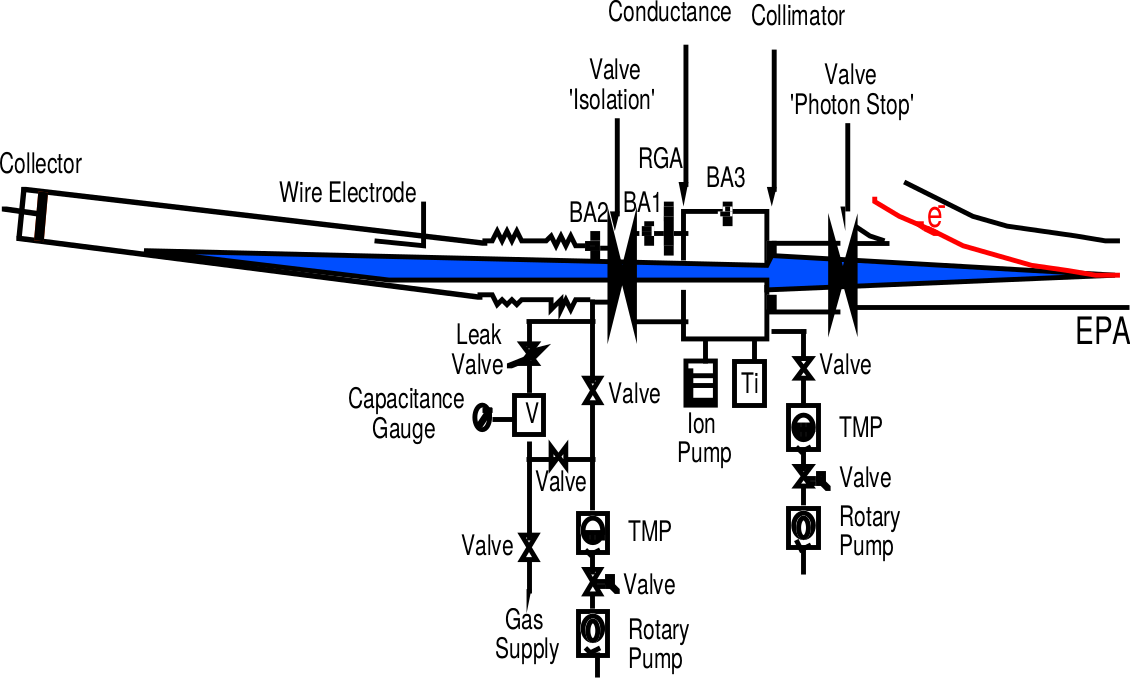
\includegraphics[width=0.8\textwidth]{../ss/experiment_baglin.png}
    \caption{Experiment setup of the paper presented in Sec.~\ref{sec:Baglin}.}
    \label{fig:exp}
\end{figure}


Fig.~\ref{fig:exp} shows the experiment setup.
It was possible to measure forward reflectivities and photoelectron yields.
The collimator is of square geometry and 11~mm wide.
The authors write:
\begin{quote}
    \small
    Due to the vertical collimation, photon energies below about 4 eV are attenuated.
\end{quote}

The photoelectrons are measured at the collector, either after direct impact or after a reflection as shown in the figure.
The ratio of the two currents is the photon reflectivity, where the backwards reflected photons are neglected (see Sec.~\ref{sec:Mahne}).

The report cites that for radiation with a critical energy of 45 and 194~eV, corresponding to 7 and 11.5~TeV LHC beams, the number of photons is multiplied by 0.46 and 0.65, respectively.
This exactly coincides with the ratio of photons above the work function with respect to all photons, see Fig.~\ref{fig:n_photons}.



\subsubsection{Results}
The results of this paper are given in Fig.~\ref{fig:baglin_table}.
Note that the photoelectrons per incident photon $Y$ has been measured, which was then transformed to the photoelectrons per absorbed photon, $Y^*$.
The reflectivity $R$ was measured at an incidence angle of 11~mrad for the sample without sawtooth.


\begin{figure}[tbh]
    \centering
    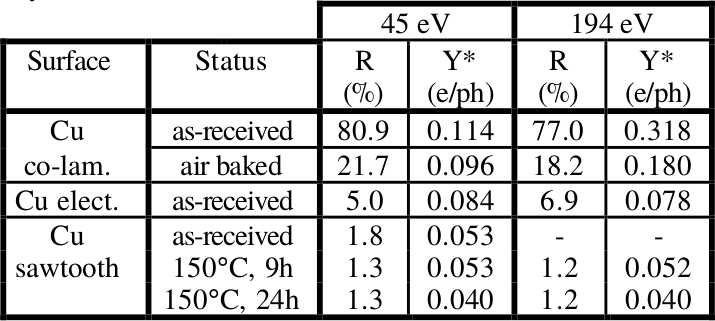
\includegraphics[width=0.4\textwidth]{../ss/baglin_table.png}
    \caption{
        The main results of the paper from Sec.~\ref{sec:Baglin}, surface properties for different materials when radiated by two different photon distributions, characterized by the critical photon energy. 
        R is the fraction of reflected photons, Y$^*$ the electron yield per absorbed photon.}
    \label{fig:baglin_table}
\end{figure}

\subsubsection{Open questions}
\begin{enumerate}
    \item
        The authors claim that the photons were sent through a collimator with 11x11~mm size, leading to the photons below 4~eV to be attenuated.
        %The resulting minimum photon energy from a maximum of 11~mm wavelengths can be calculated.
        %\begin{align}
        %    E = \frac{ch}{\lambda} = 1.2\cdot10^{-4}~\text{eV}
        %\end{align}
        %In order to attenuate photon energies below 4 eV, the collimation would have to be about 0.2~$\mu$m.
        It is not clear how exactly the low energy photons were attenuated, or why this would have been necessary.
    \item
        The photon induced scrubbing of the surface was not subject of this paper.
        The photon flux or integrated photon dose is not stated.
        The photoelectron yields that are quantified in this paper should probably be used as an upper limit.
    \item
        Considering the paper from Sec.~\ref{sec:Mahne}, the real reflectivity of the samples, especially with sawtooth, is expected to be higher.
        Because $Y^*$ and $R$ are not independent, $Y^*$ should maybe be updated (increased) according to Eq.~(\ref{eq:yy}).
\end{enumerate}

